% Options for packages loaded elsewhere
\PassOptionsToPackage{unicode}{hyperref}
\PassOptionsToPackage{hyphens}{url}
\PassOptionsToPackage{dvipsnames,svgnames,x11names}{xcolor}
%
\documentclass[
  number,
  preprint,
  3p]{elsarticle}

\usepackage{amsmath,amssymb}
\usepackage{iftex}
\ifPDFTeX
  \usepackage[T1]{fontenc}
  \usepackage[utf8]{inputenc}
  \usepackage{textcomp} % provide euro and other symbols
\else % if luatex or xetex
  \usepackage{unicode-math}
  \defaultfontfeatures{Scale=MatchLowercase}
  \defaultfontfeatures[\rmfamily]{Ligatures=TeX,Scale=1}
\fi
\usepackage{lmodern}
\ifPDFTeX\else  
    % xetex/luatex font selection
\fi
% Use upquote if available, for straight quotes in verbatim environments
\IfFileExists{upquote.sty}{\usepackage{upquote}}{}
\IfFileExists{microtype.sty}{% use microtype if available
  \usepackage[]{microtype}
  \UseMicrotypeSet[protrusion]{basicmath} % disable protrusion for tt fonts
}{}
\makeatletter
\@ifundefined{KOMAClassName}{% if non-KOMA class
  \IfFileExists{parskip.sty}{%
    \usepackage{parskip}
  }{% else
    \setlength{\parindent}{0pt}
    \setlength{\parskip}{6pt plus 2pt minus 1pt}}
}{% if KOMA class
  \KOMAoptions{parskip=half}}
\makeatother
\usepackage{xcolor}
\setlength{\emergencystretch}{3em} % prevent overfull lines
\setcounter{secnumdepth}{5}
% Make \paragraph and \subparagraph free-standing
\ifx\paragraph\undefined\else
  \let\oldparagraph\paragraph
  \renewcommand{\paragraph}[1]{\oldparagraph{#1}\mbox{}}
\fi
\ifx\subparagraph\undefined\else
  \let\oldsubparagraph\subparagraph
  \renewcommand{\subparagraph}[1]{\oldsubparagraph{#1}\mbox{}}
\fi


\providecommand{\tightlist}{%
  \setlength{\itemsep}{0pt}\setlength{\parskip}{0pt}}\usepackage{longtable,booktabs,array}
\usepackage{calc} % for calculating minipage widths
% Correct order of tables after \paragraph or \subparagraph
\usepackage{etoolbox}
\makeatletter
\patchcmd\longtable{\par}{\if@noskipsec\mbox{}\fi\par}{}{}
\makeatother
% Allow footnotes in longtable head/foot
\IfFileExists{footnotehyper.sty}{\usepackage{footnotehyper}}{\usepackage{footnote}}
\makesavenoteenv{longtable}
\usepackage{graphicx}
\makeatletter
\def\maxwidth{\ifdim\Gin@nat@width>\linewidth\linewidth\else\Gin@nat@width\fi}
\def\maxheight{\ifdim\Gin@nat@height>\textheight\textheight\else\Gin@nat@height\fi}
\makeatother
% Scale images if necessary, so that they will not overflow the page
% margins by default, and it is still possible to overwrite the defaults
% using explicit options in \includegraphics[width, height, ...]{}
\setkeys{Gin}{width=\maxwidth,height=\maxheight,keepaspectratio}
% Set default figure placement to htbp
\makeatletter
\def\fps@figure{htbp}
\makeatother

\makeatletter
\makeatother
\makeatletter
\makeatother
\makeatletter
\@ifpackageloaded{caption}{}{\usepackage{caption}}
\AtBeginDocument{%
\ifdefined\contentsname
  \renewcommand*\contentsname{Table of contents}
\else
  \newcommand\contentsname{Table of contents}
\fi
\ifdefined\listfigurename
  \renewcommand*\listfigurename{List of Figures}
\else
  \newcommand\listfigurename{List of Figures}
\fi
\ifdefined\listtablename
  \renewcommand*\listtablename{List of Tables}
\else
  \newcommand\listtablename{List of Tables}
\fi
\ifdefined\figurename
  \renewcommand*\figurename{Figure}
\else
  \newcommand\figurename{Figure}
\fi
\ifdefined\tablename
  \renewcommand*\tablename{Table}
\else
  \newcommand\tablename{Table}
\fi
}
\@ifpackageloaded{float}{}{\usepackage{float}}
\floatstyle{ruled}
\@ifundefined{c@chapter}{\newfloat{codelisting}{h}{lop}}{\newfloat{codelisting}{h}{lop}[chapter]}
\floatname{codelisting}{Listing}
\newcommand*\listoflistings{\listof{codelisting}{List of Listings}}
\makeatother
\makeatletter
\@ifpackageloaded{caption}{}{\usepackage{caption}}
\@ifpackageloaded{subcaption}{}{\usepackage{subcaption}}
\makeatother
\makeatletter
\@ifpackageloaded{tcolorbox}{}{\usepackage[skins,breakable]{tcolorbox}}
\makeatother
\makeatletter
\@ifundefined{shadecolor}{\definecolor{shadecolor}{rgb}{.97, .97, .97}}
\makeatother
\makeatletter
\makeatother
\makeatletter
\makeatother
\journal{Journal Name}
\ifLuaTeX
  \usepackage{selnolig}  % disable illegal ligatures
\fi
\usepackage[]{natbib}
\bibliographystyle{elsarticle-num}
\IfFileExists{bookmark.sty}{\usepackage{bookmark}}{\usepackage{hyperref}}
\IfFileExists{xurl.sty}{\usepackage{xurl}}{} % add URL line breaks if available
\urlstyle{same} % disable monospaced font for URLs
\hypersetup{
  pdftitle={Using Conditional Autoregression to Model Tuberculosis Dynamics in Ca Mau Province},
  pdfauthor={Viet Long Bui; Romain Ragonnet; Gregory Fox; James M. Trauer},
  pdfkeywords={CAR, TB},
  colorlinks=true,
  linkcolor={blue},
  filecolor={Maroon},
  citecolor={Blue},
  urlcolor={Blue},
  pdfcreator={LaTeX via pandoc}}

\setlength{\parindent}{6pt}
\begin{document}

\begin{frontmatter}
\title{Using Conditional Autoregression to Model Tuberculosis Dynamics
in Ca Mau Province \\\large{Conditional Autoregression to Model
Tuberculosis Dynamics in Ca Mau} }
\author[1]{Viet Long Bui%
\corref{cor1}%
}
 \ead{viet.bui1@monash.edu} 
\author[1]{Romain Ragonnet%
%
}
 \ead{romain.ragonnet@monash.edu} 
\author[2]{Gregory Fox%
%
}
 \ead{greg.fox@sydney.edu.au} 
\author[]{James M. Trauer%
%
}
 \ead{james.trauer@monash.edu} 

\affiliation[1]{organization={Epidemiological Modelling Unit, School of
Public Health and Preventive Medicine, Monash
University},,postcodesep={}}
\affiliation[2]{organization={University of Sydney},,postcodesep={}}

\cortext[cor1]{Corresponding author}




        
\begin{abstract}
This is the abstract.
\end{abstract}





\begin{keyword}
    CAR \sep 
    TB
\end{keyword}
\end{frontmatter}
    \ifdefined\Shaded\renewenvironment{Shaded}{\begin{tcolorbox}[enhanced, interior hidden, frame hidden, sharp corners, borderline west={3pt}{0pt}{shadecolor}, breakable, boxrule=0pt]}{\end{tcolorbox}}\fi

\hypertarget{introduction}{%
\section{Introduction}\label{introduction}}

Tuberculosis (TB) remains a critical concern in global health
\citep{villar-hernandez-2023}. Its transmission typically occurs within
close communities, such as families, emphasizing the need for a deep
understanding of its dynamics at a local level to devise effective
interventions \citep{cole-2020}.\\
In the southernmost province of Vietnam, Ca Mau, TB remains a major
health issue. The notification rate of approximately 120 cases per
100,000 individuals underscores the substantial difficulty in
controlling the disease. Despite ongoing efforts, TB continues to impact
the health of the local population, influenced by factors like
socio-economic conditions, healthcare accessibility, and environmental
elements. Gaining a comprehensive understanding of TB dynamics in Ca Mau
is vital for formulating more effective disease management and control
strategies.\\
Originating from Besag, York, and Mollié's 1991 research
\citep{besag-1991}, CAR models are particularly adept at handling
spatial dependencies, a frequent aspect in the spread of diseases. This
capability makes them highly valuable in epidemiological studies where
understanding spatial disease patterns is crucial. CAR models are
particularly relevant in modeling infectious diseases such as TB, where
geographical and social proximity plays a crucial role in transmission.
Research by Lee in 2011 highlights the capability of CAR models in
pinpointing high-risk areas and deciphering spatial disease patterns
\citep{lee-2011}. Their application in TB epidemiology is gaining
recognition for its ability to tackle the complexity of TB transmission
\citep{lima-2019}. These models provide insight into the interaction
between TB spread and spatially-structured social and environmental
factors.

\begin{figure}

{\centering 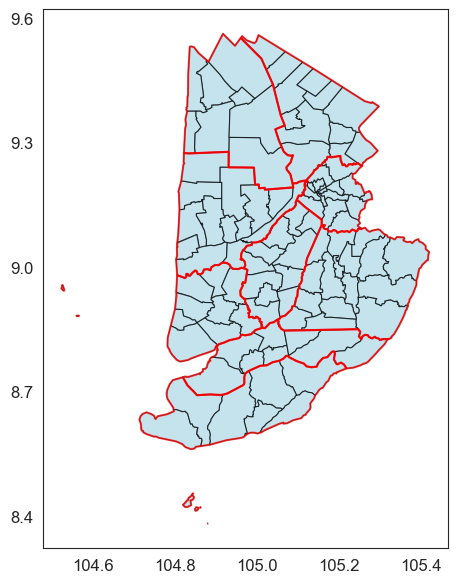
\includegraphics{docs_files/figure-pdf/camap_map-output-1.png}

}

\caption{A map of Ca Mau Province}

\end{figure}

\hypertarget{research-objectives}{%
\section{Research objectives:}\label{research-objectives}}

Primary Objective: To apply a Conditional Autoregressive (CAR) model to
analyze and understand the spatial dynamics of Tuberculosis (TB) in Ca
Mau Province, Vietnam. This includes:\\
1. Mapping TB incidence to identify high-prevalence areas.\\
2. Investigating socio-economic, environmental, and healthcare factors
influencing TB distribution.\\
3. Utilizing CAR models to predict TB transmission patterns.\\
4. Providing data-driven insights for local TB control and prevention
strategies.

\hypertarget{methodology}{%
\section{Methodology}\label{methodology}}

\begin{enumerate}
\def\labelenumi{\arabic{enumi}.}
\tightlist
\item
  Data Collection:\\
\end{enumerate}

\begin{itemize}
\tightlist
\item
  Data Sources: TB Notification will be collected from the NTP,
  demographic and population will be collected from Camau Statistical
  Office. Map will be collected from GADM website.\\
\item
  Time Frame: From 2011 - to 2022.\\
\end{itemize}

\begin{enumerate}
\def\labelenumi{\arabic{enumi}.}
\setcounter{enumi}{1}
\tightlist
\item
  Model Development and Implementation:\\
\end{enumerate}

\begin{itemize}
\tightlist
\item
  Conditional Autoregressive (CAR) Model: Develop a CAR model tailored
  to the spatial epidemiology of TB in Ca Mau Province.\\
\item
  Variable Selection: Include variables such as population density,
  socio-economic status, healthcare access, and environmental factors.\\
\item
  Model Calibration: Fine-tune the model parameters using a subset of
  the data to ensure accurate representation of local TB dynamics.\\
\end{itemize}

\begin{enumerate}
\def\labelenumi{\arabic{enumi}.}
\setcounter{enumi}{2}
\tightlist
\item
  Statistical Analysis:\\
\end{enumerate}

\begin{itemize}
\tightlist
\item
  Software: Use statistical software R for data analysis and model
  implementation.
\item
  Spatial Analysis: Conduct spatial analysis to identify hotspots and
  patterns in TB occurrence.
\item
  Sensitivity Analysis: Perform sensitivity analysis to assess the
  robustness of the model against variations in input parameters.\\
\end{itemize}

\begin{enumerate}
\def\labelenumi{\arabic{enumi}.}
\setcounter{enumi}{3}
\tightlist
\item
  Model Validation:\\
\end{enumerate}

\begin{itemize}
\tightlist
\item
  Validation Techniques: Use cross-validation methods to test the
  model's predictive accuracy.\\
\item
  Comparison with Traditional Models: Compare the CAR model's results
  with those obtained from traditional epidemiological models to
  evaluate performance improvements.\\
\end{itemize}

\begin{enumerate}
\def\labelenumi{\arabic{enumi}.}
\setcounter{enumi}{4}
\tightlist
\item
  Interpretation and Application:\\
\end{enumerate}

\begin{itemize}
\tightlist
\item
  Insight Generation: Interpret the model outputs to identify key
  drivers of TB in Ca Mau Province.\\
\item
  Policy Recommendations: Formulate recommendations for TB control and
  prevention based on model findings.
\end{itemize}

\hypertarget{expected-results}{%
\section{Expected results:}\label{expected-results}}

Identification of localized spatial clusters indicating high and low TB
incidence rates within An Giang Province using CAR models. Exploration
of fluctuations and potential patterns in TB transmission over time,
offering insights into temporal dynamics. Analysis of associations
between TB incidence rates and demographic factors sourced from the An
Giang statistical yearbook.

\hypertarget{data-governance-and-ethics}{%
\section{Data Governance and Ethics:}\label{data-governance-and-ethics}}

The dataset that contains the aggregated data of patients of new and
relapse patients with all forms of TB, notified in Nam Dinh, in the
5-year age group and sex at communal level from 2011 to 2022 will be
obtained from the Vietnam NTP. Acquisition of this data is expected to
require a low-risk ethics approval from Monash University, ensuring
compliance with ethical guidelines. The aggregated nature of the dataset
mandates its secure storage, in accordance Monash University's
guidelines.


\renewcommand\refname{References}
  \bibliography{tbbib.bib}


\end{document}
